\section{Case Study} \label{CaseStudy}
\begin{table*}[h!]
\centering
\resizebox{1\textwidth}{!}{
\begin{tabular}{clclcc}
\toprule
Test ID & Test description (See Fig \ref{Test_a} and \ref{Test_b}) & Collision/Intersection & Collision Type & Look ahead distance (m) & No. of repeats \\ \midrule
1       & Two vehicles driving                   & No  & N/A & 2 & 1000 \\
2       & Two vehicles driving                   & Yes & Vehicle and Vehicle & 2 & 1000 \\
3       & Two vehicles driving and a pedestrian  & No  & N/A & 2 & 1000 \\
4       & Two vehicles driving and a pedestrian  & Yes & Vehicle and Pedestrian & 2 & 1000 \\
5       & Two pedestrians                        & No  & N/A & 2 & 1000 \\
6       & Two pedestrians                        & Yes & Pedestrian and Pedestrian & 0.4 & 1000 \\
7       & Two pedestrians                        & Yes & Pedestrian and Pedestrian & 2 & 1000 \\
8       & Two pedestrians                        & Yes & Pedestrian and Pedestrian & 20 & 1000 \\
\bottomrule
\end{tabular}
}
\caption{Set of experiments}
\label{TableOfExperiments}
\end{table*}

\noindent Given that our interest is on CAV simulations, this study presents a number of experiments run on typical agents used in CAV simulations and their interactions with each other. These agents are classified into two, either vehicles(cars, motorcycles, bikes etc.) or pedestrians (can include animals). \\\\
Here we will walk through our hypothesis, description of our tests and the analysis of results from the different tests. We will point out at each stage where we sit in Fig \ref{method_diagram} as we go through this case study.    

\subsection{Problem And Hypothesis}
\noindent We want to see whether using Unreal Engine 4 (UE4) along with CARLA \cite{CARLA_paper} for V\&V of CAV simulations is deterministic or not; if not then what is the level of non-determinism we will operate with, is it acceptable or not, and whether it worsens with stressing GPU and CPU.\\\\
Our hypothesis is that since UE4 is a gaming engine it will not be deterministic, however, the level of non-determinism would be very low to acceptable limits that allows verification engineers to use it confidently.
This behaviour is expected not to hold as the level of computing stress increases.     

\begin{figure}[h]
    \centering
    \begin{subfigure}{.24\textwidth}
        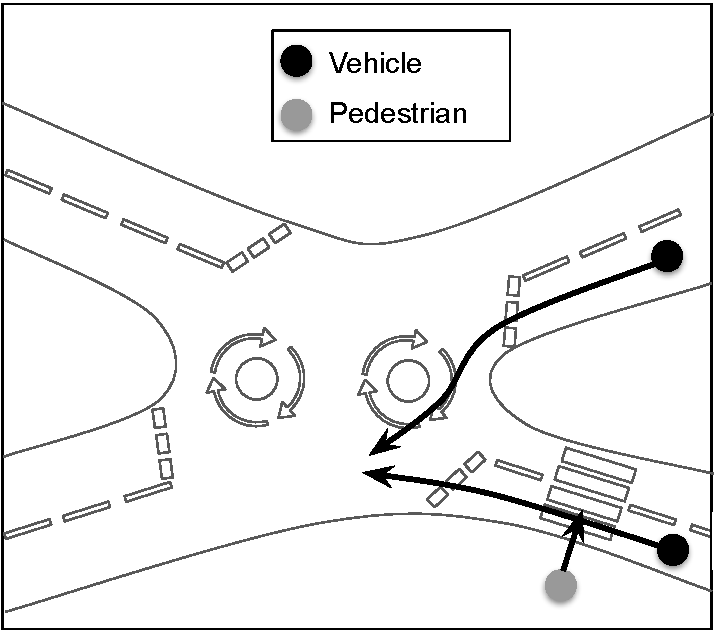
\includegraphics[width=1\textwidth]{Other/Figures/TestCasesDiagram_a.pdf}
        \caption{}
        \label{Test_a}
    \end{subfigure}
    \begin{subfigure}{.24\textwidth}
        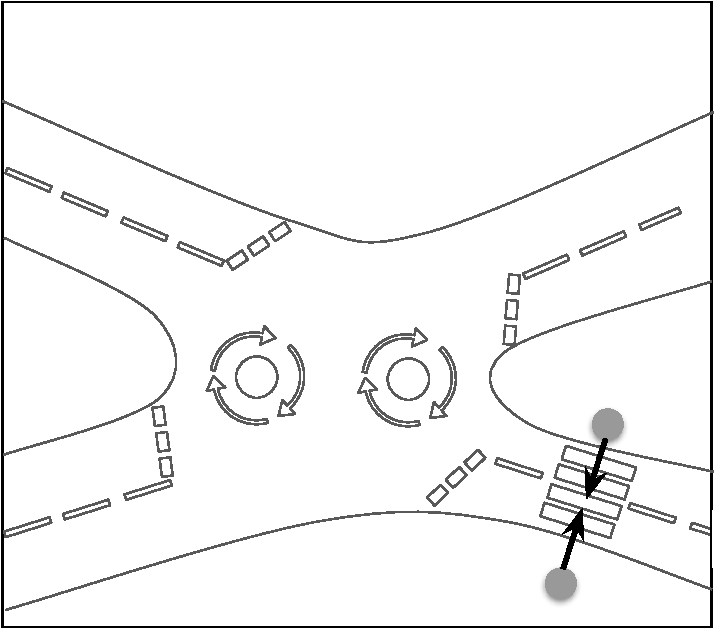
\includegraphics[width=1\textwidth]{Other/Figures/TestCasesDiagram_b.pdf}
        \caption{}
        \label{Test_b}
    \end{subfigure}
    \caption{Shows the setup of the different tests in Table \ref{TableOfExperiments} (a)Test IDs 1 to 4 (b)Test IDs 5 to 8.}
\end{figure}

\begin{figure}[h]
    \centering
    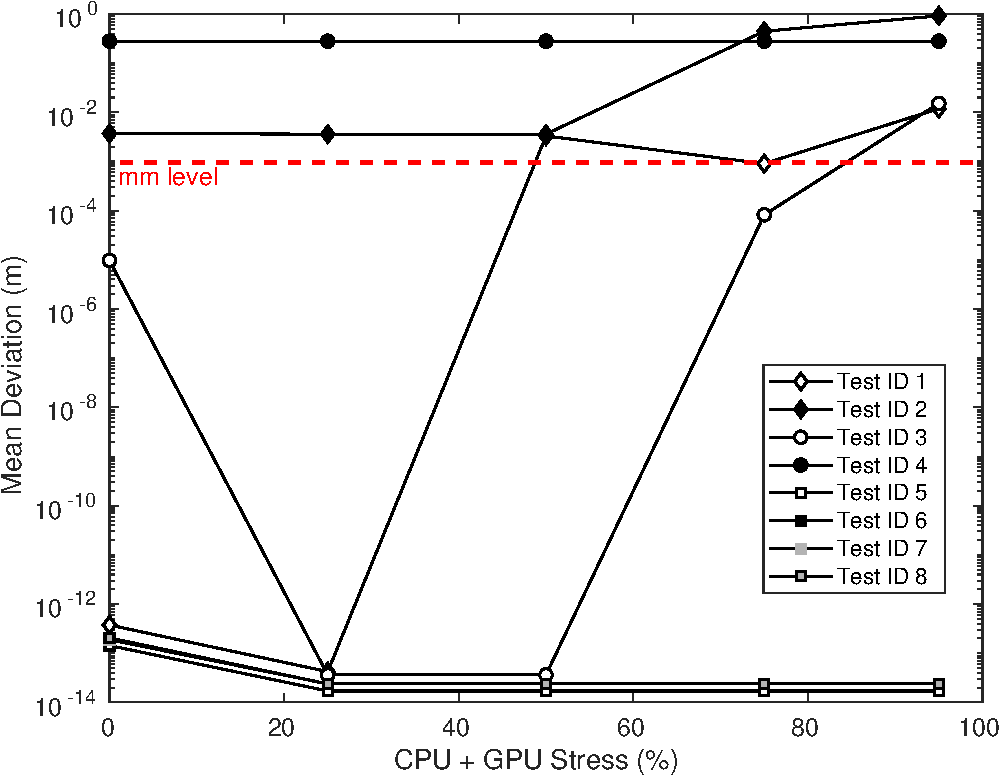
\includegraphics[width=0.48\textwidth]{Other/Figures/ExperimentsStressSummary.pdf}
    \caption{Summary of mean deviation for the different tests runs plotted against the different CPU+GPU stresses.}

    \label{ExperimentsStressSummary}
\end{figure}
\subsection{Tests Description And Technicalities}\label{TestsDescriptionAndTechnicalities}
\noindent The vehicles in this simulator follow a trajectory of waypoints using a PID controller and they have a look ahead distance that they target for from a given list of trajectory waypoints. 
Similarly with the pedestrians, but they don't have a PID controller and they can do dynamic path planning using A* algorithm to reach their destination or in this case a trajectory waypoint.\\\\ 
\noindent Starting from step 1 in the methodology diagram (Design Experiment); we are using a double mini roundabout for our experiments. 
The list of tests shown in Table \ref{TableOfExperiments} were chosen to cover the mandatory interactions between the different types of agents. 
These are summed up in the following: \textbf{i)}Agents (vehicles and pedestrians) moving with no collisions or interactions with each other \textbf{ii)}Collision between vehicles \textbf{iii)}Collision (intersection) between pedestrians \textbf{iv)}Collision between vehicles and pedestrians.\\\\
\noindent Tests 1, 3and 5 are similar and there are no collisions in them, they were done as separate tests (instead of combining them into one) for the sake of simplicity and to use them as base lines for the tests-collision versions of them. The tests for collisions and non-collisions differ by a very slight change in the trajectory of the agents just to make them avoid colliding or intersecting with each other. \\\\ 
Test 2 is a collision between two vehicles and no pedestrians involved and is depicted by \ref{Test_a}, where the two vehicles will approach the roundabout and crash.\\\\
Tests 6,7 and 8 are tests with pedetrians having the same trajectory waypoints but walking in opposite directions to each other (see Fig \ref{Test_b}). 
Pedestrians have the functionality of dynamic path planning i.e. they can avoid obstacles to reach their waypoints and so they can avoid bumping into each other. 
Hence, to make sure they intersect (collide) with each other then we  have set tests 6,7 and 8 to be the same but with different look ahead distances; the smaller the look ahead distance the less chance they will get to path plan around each other, and thus making sure they intersect.\\\\ 
In V\&V of CAV simulations, collisions of pedestrians together is not of much interest, nevertheless we decided to include these tests for the sake of completeness and to obtain a full image of the level of non-determinism of the simulator.\\\\
Test 4, is where a vehicle hits a pedestrian and runs over it on a zebra line, as shown in Fig \ref{Test_a}.\\\\
Proceeding to step 2; by doing various inspections around the different internal settings of this simulator we did not notice any improvement or worsening in the results. 
On the other hand the external settings (step 3) did show significant variations on the results as will be discussed in the next section. \\\\
Different levels of stress were applied to the computer; using the ------ to stress the CPU and ------ for the GPU.\\\\ 
In terms of running the experiments (step 4), \textbf{i)} the specs of the computer used are -----; \textbf{ii)} ------ was used to monitor the levels of GPU and CPU stress before and while the experiment was executed; \textbf{iii)} the computer was left alone and not used for any other tasks while the runs were executed.

\subsection{Results And Discussion}
\begin{figure*}[h]
    \centering
    \begin{subfigure}{.49\textwidth}
        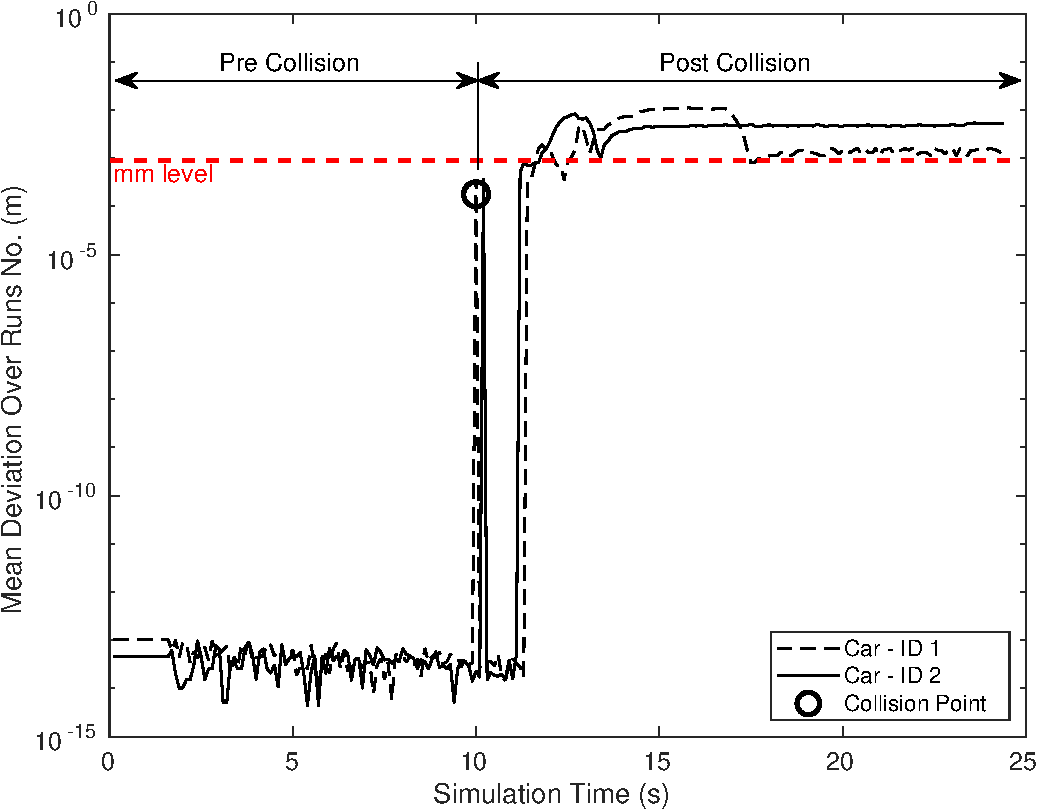
\includegraphics[width=1\textwidth]{Other/Figures/CarsCollisionCG25.pdf}
        \caption{}
        \label{CarsCollisionCG25}
    \end{subfigure}
    \begin{subfigure}{.49\textwidth}
        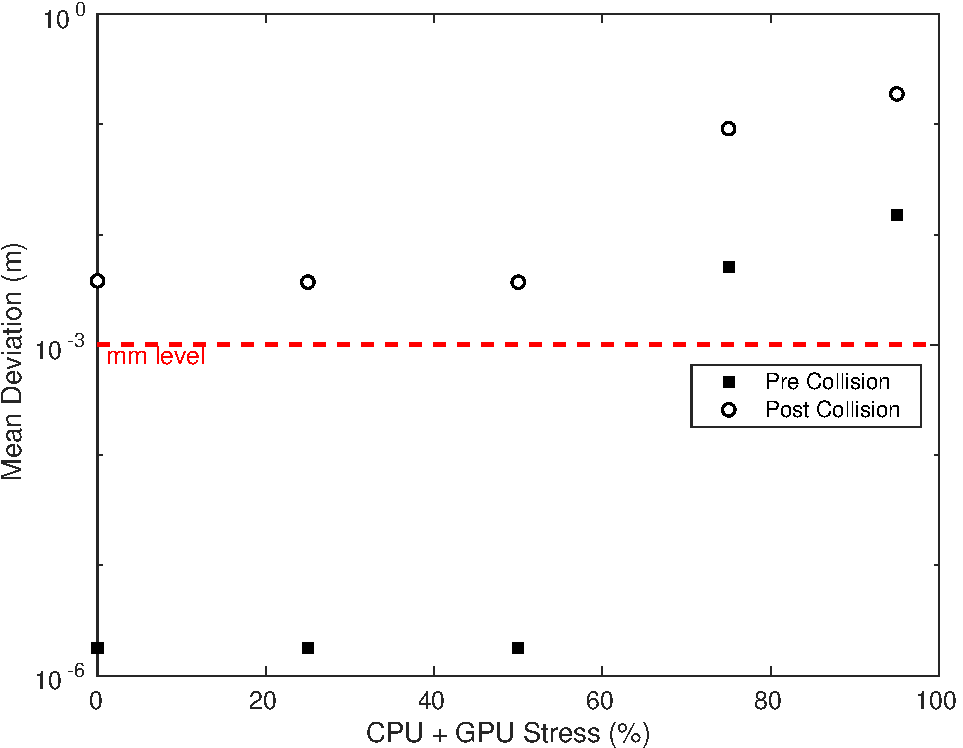
\includegraphics[width=1\textwidth]{Other/Figures/CarsCollisionPrePost.pdf}
        \caption{}
        \label{CarsCollisionPrePost}
    \end{subfigure}
    \caption{Test ID 2 (a)Mean deviation vs simulation time for 25\% stress. (b)Pre and post collision mean deviation at different CPU+GPU stresses.}
\end{figure*}

\begin{figure*}[h]
    \centering
    \begin{subfigure}{.49\textwidth}
        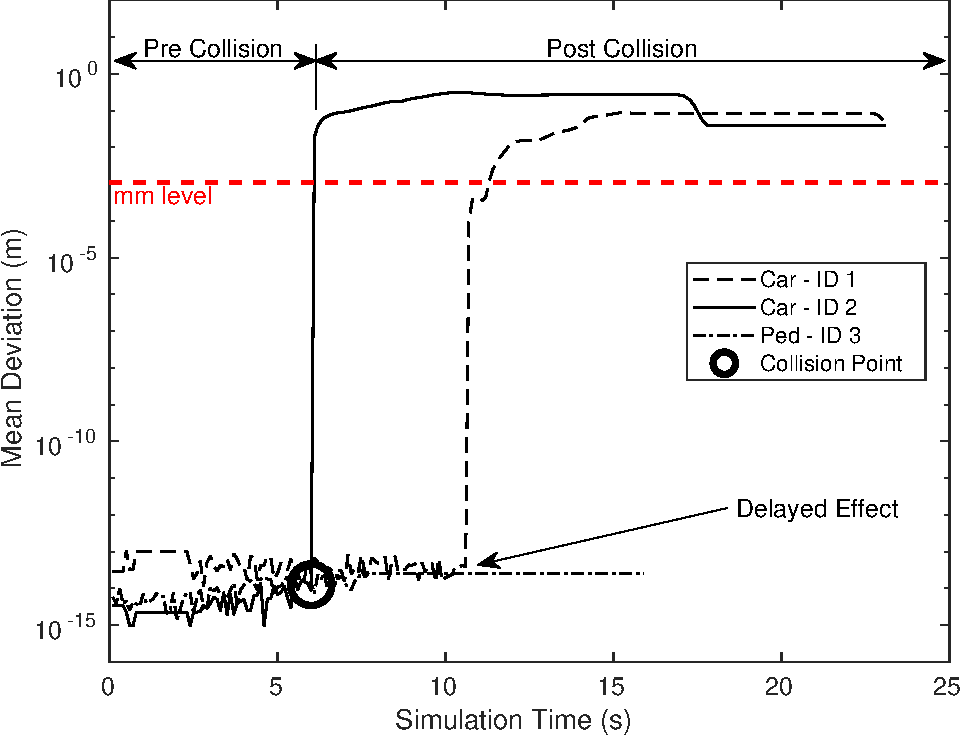
\includegraphics[width=1\textwidth]{Other/Figures/CarsPeopleCollsionsCG25.pdf}
        \caption{}
        \label{CarsPeopleCollsionsCG25}
    \end{subfigure}
    \begin{subfigure}{.49\textwidth}
        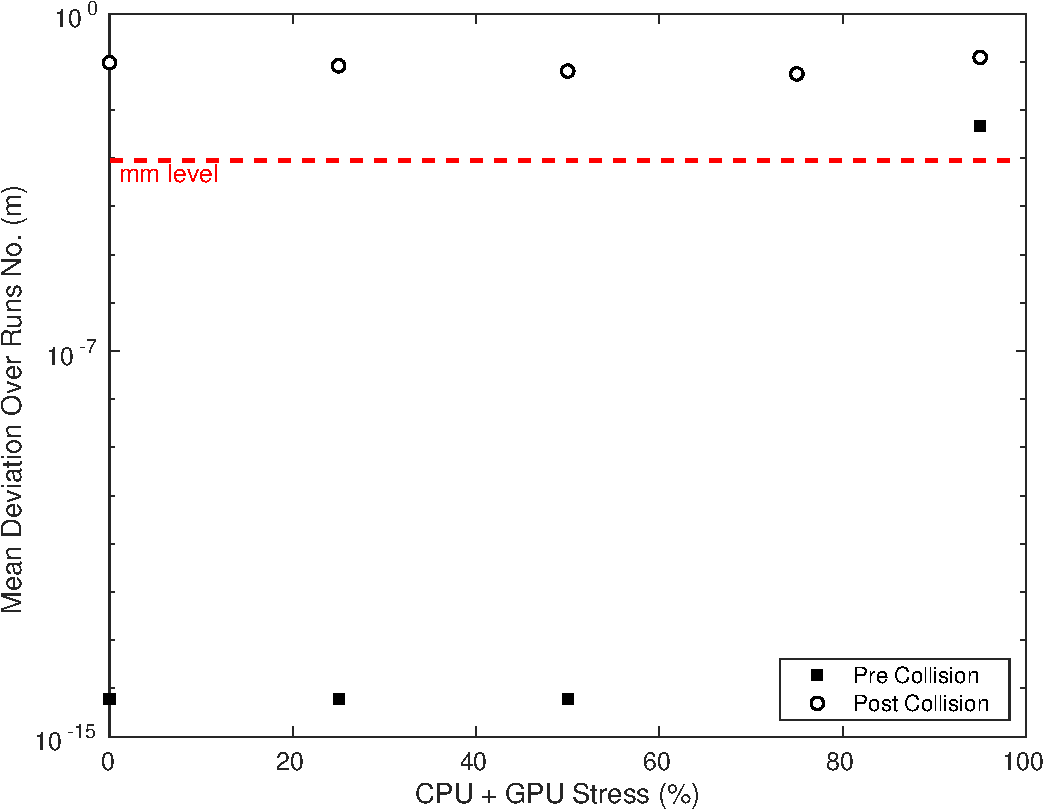
\includegraphics[width=1\textwidth]{Other/Figures/CarsPeopleCollisionPrePost.pdf}
        \caption{}
        \label{CarsPeopleCollisionPrePost}
    \end{subfigure}
    \caption{Test ID 4 (a)Mean deviation vs simulation time for 25\% stress. (b)Pre and post collision mean deviation at different CPU+GPU stresses.}
\end{figure*}
\noindent We start by analysing (step 5) the summary from all of the tests plotted in Fig \ref{ExperimentsStressSummary}. 
Note the dotted red line in the plot shows the millimeter (mm) level. 
Below this level we assume that the level of non-determinism is very low for V\&V of CAV simulations purposes, that it is sufficient to assume the tests are deterministic. 
This line can be moved up or down and it is entirely up to verification engineers where they want to define the level below which tests are assumed to be sufficiently deterministic, but just for the sake of argument we chose it to be the millimeter level.\\\\
First, the tests with no collisions are considered, these represent tests 1, 3 and 5.
Tests 1 and 3, which involves vehicles only and vehicles with pedestrians respectively, shows to be deterministic for stress levels below 50\% and as the stress level increases they surpass the red line crossing our defined deterministic level but still being sufficiently low (i.e. with in the centimeter level). This clearly shows how the load on a computer (i.e. stressing CPU and GPU) can have drastic effects on the repeatablitiy of tests.
This is more specific to vehicle agents rather than pedestrians since the behaviour of pedestrians is consistent and remarkably below the mm level for all of the different levels of stress shown by test 5, where only pedestrians are involved with no collisions, from which it can be deduced that the mean deviation change with the stress level in test 3 was solely due to the vehicles. \\\\
Next, given the pedestrians were showing a very robust and low level of non-determinism behaviour, we ran tests for pedestrians colliding (i.e. with paths intersection) for different look ahead distances to exploit whether that would cause any changes, but yet as it can be seen by lines Test IDs' 6,7 and 8 that their performance is consistent for all of the different tests.


\noindent Finally, we look at the other collisions tests, tests 2 and 4 where the tests correspond to a collision between two vehicles and a collision between a vehicle and a pedestrian respectively. 
We observe that in both of these tests the mean deviation is always above our red line regardless of the stress level, nevertheless still increasing the stress levels shows worsening effects. \\\\
\noindent Thus, we resorted to plotting the mean deviation of these two tests vs simulation time with stress level \%25 chosen arbitrarily (see Fig. \ref{CarsCollisionCG25} and \ref{CarsPeopleCollsionsCG25}). 
Doing that we discovered that after collisions occur there is a jump in the mean deviation, which is what causes the averaged mean deviation through the whole simulation time in Fig \ref{ExperimentsStressSummary} to always surpass our red line.\\\\
\noindent Plotting Figs \ref{CarsCollisionPrePost} and \ref{CarsPeopleCollisionPrePost}, which shows the mean deviation pre and post collision for the different stress levels; it can be seen that there is two discrete levels for the pre and post collison devaition from these plots and as the stress increases these two discrete levels start to merge. 
However, in V\&V of CAV simualtions we  are normally interested in the point until a collision occur after which the simulation will be terminated. Thus, the post collision effect should not be of much concern in the context of CAVs.\\\\
\noindent It is important to note, however, that in test 4 a delayed effect of increase in the level of non determinism was noticed to Car ID 1, which interestingly was not involved in the collision, this was attributed to how the physics engine was programmed to calculate collisions which might cause other obscure behaviours to other agents. The importance of this outcome is that it shows even if the ego vehicle is not involved in a collision, but other agents are, this will still have effects on the determinism of the ego vehicle. Thus failing to stay below our red line and the test should be terminated.

% \noindent\underline{\textit{No collisions:}}
% First, the tests with no collsions are considered, these represnt tests' ID 1, 3 and 5. ...
% --General deterministic behaviour of all of the agnets whent there are no collisions (tests 1,3 and 5)\\\\
% \noindent\underline{\textit{Pedestrians paths intersection:}}
% Pedestrians do not just blindly follow their trajectories, as already iterated in section \ref{TestsDescriptionAndTechnicalities}; thus it it 
% --Pathintersections bewteen pedestrains (tests 6,7 and 8)\\\\
% \noindent\underline{\textit{Collision between vehicles:}}
% Test 2 where the vehilcles collide together...
% --Collsion between vehicles alone (test 2)\\\\

% \noindent\underline{\textit{Collision between vehicles and pedestrians:}}
% --collsion between vehicles and pedestrains(test 4)
% -- coparison between variance before and after collsion


% - after a collsion the level of non determinsim increases significantly 
% - However In V\&V of CAV simulations, if a collsion is detected then the test should end

\TODO{We might need to change the y axes nameing betweent he summary plot (fig 4) and the fig 5 and 6, to show that one is mean deviation of all runs and thourgh out simulation time and the other is only between the different runs.}

\noindent In summary, from the tests carried out we can deduce that for a computer of the following specifications,-----..--, that all tests carried out using CARLA in UE4 are gauranteed to be deterministic and repeatable (according to our definition by the red line) as long as the CPU + GPU stress does not exceed 50\% and tests are terminated as soon as a collision of any type is detected in the simulation. 